
%%%%%%%%%%%%%%%%%%%%%%%%%%%%%%%%%%%%%%%%%%%%%%
\section{Photon detection system}
\label{sec:pd_system}

\fixme{This section still needs work (Anne 8/18}

The scope of the photon detector system (PDS) for the DUNE far detector
reference design includes design, procurement, fabrication,
testing, delivery and installation of the following components:
\begin{itemize}
\item light collection system including wavelength shifter and light guides,
\item silicon photo-multipliers (SiPMs),
\item readout electronics,
\item calibration system, and
\item related infrastructure (frames, mounting boards, etc.).
\end{itemize}

\fixme{I suggest adding purpose and requirements here, i.e., some info from what was put in the calibration section:

The current DUNE far detector designs are anticipated to have sufficient sensitivity to provide event timing information for atmospheric neutrino and proton decay channels, but sufficient efficiency down to the 5 MeV neutrino energy level desired by the supernova program has to be demonstrated in future designs.
In the absence of precise physics requirements for the PDS and in order to support R\&D activities on the PD development it was decided that the PDS should provide a time stamp to determine the time of occurrence of an event (so called \textit{time zero}) with an accuracy much better than 30~ns.
}

LAr is an excellent scintillating medium and the photon detection
system will exploit this property in the far detector.  With an
average energy of 19.5~eV needed to produce a photon (at zero field),
a typical particle depositing 1~MeV in LAr will generate
40,000~photons with wavelength of 128~nm. At higher fields this will
be reduced, but at 500~V/cm the yield is still $\sim$20,000~photons
per MeV. Roughly 1/4 of the photons are promptly emitted with a
lifetime of about 6~ns while the rest have a lifetime of
1100--1600~ns. Prompt and delayed photons are detected in
  precisely the same way by the photon detection system. LAr is
highly transparent to the 128-nm VUV photons with a Rayleigh
scattering length of (66~$\pm$~3)~cm~\cite{Rayleigh} and absorption
length of $>$200~cm; this attenuation length requires a LN$_2$
  content of less than 20~ppm. The relatively large light yield makes
the scintillation process an excellent candidate for determination of
$t_0$ for non-beam related events. Detection of the scintillation
light may also be helpful in background rejection and triggering on
non-beam events.

The photon detection system reference design described in this section
meets the required performance for light collection for the DUNE far
detector. This includes detection of light from proton decay
candidates (as well as beam neutrino events) with high efficiency to
enable 3D spatial localization of candidate events. The TPC will
provide supernova neutrino detection. 
The photon system will provide the $t_0$ timing of
events relative to TPC timing with a resolution better than 1~$\mu$s
(providing position resolution along the drift direction of a couple of mm). 

Figure~\ref{fig:PD_overview} shows the layout for the photon detector
system described in this section. %, which will be described in the following sections.
\begin{cdrfigure}[Photon detection system overview]{PD_overview}{Overview of the PDS
    system showing a cartoon schematic (a) of a single PDS module
    in the LAr and the channel ganging scheme used to reduce the
    number of readout channels. Panel (b) shows how each PDS module
    will be inserted into an APA frame. There will be 10 photon detectors (PDs) inserted
    into an APA frame.}
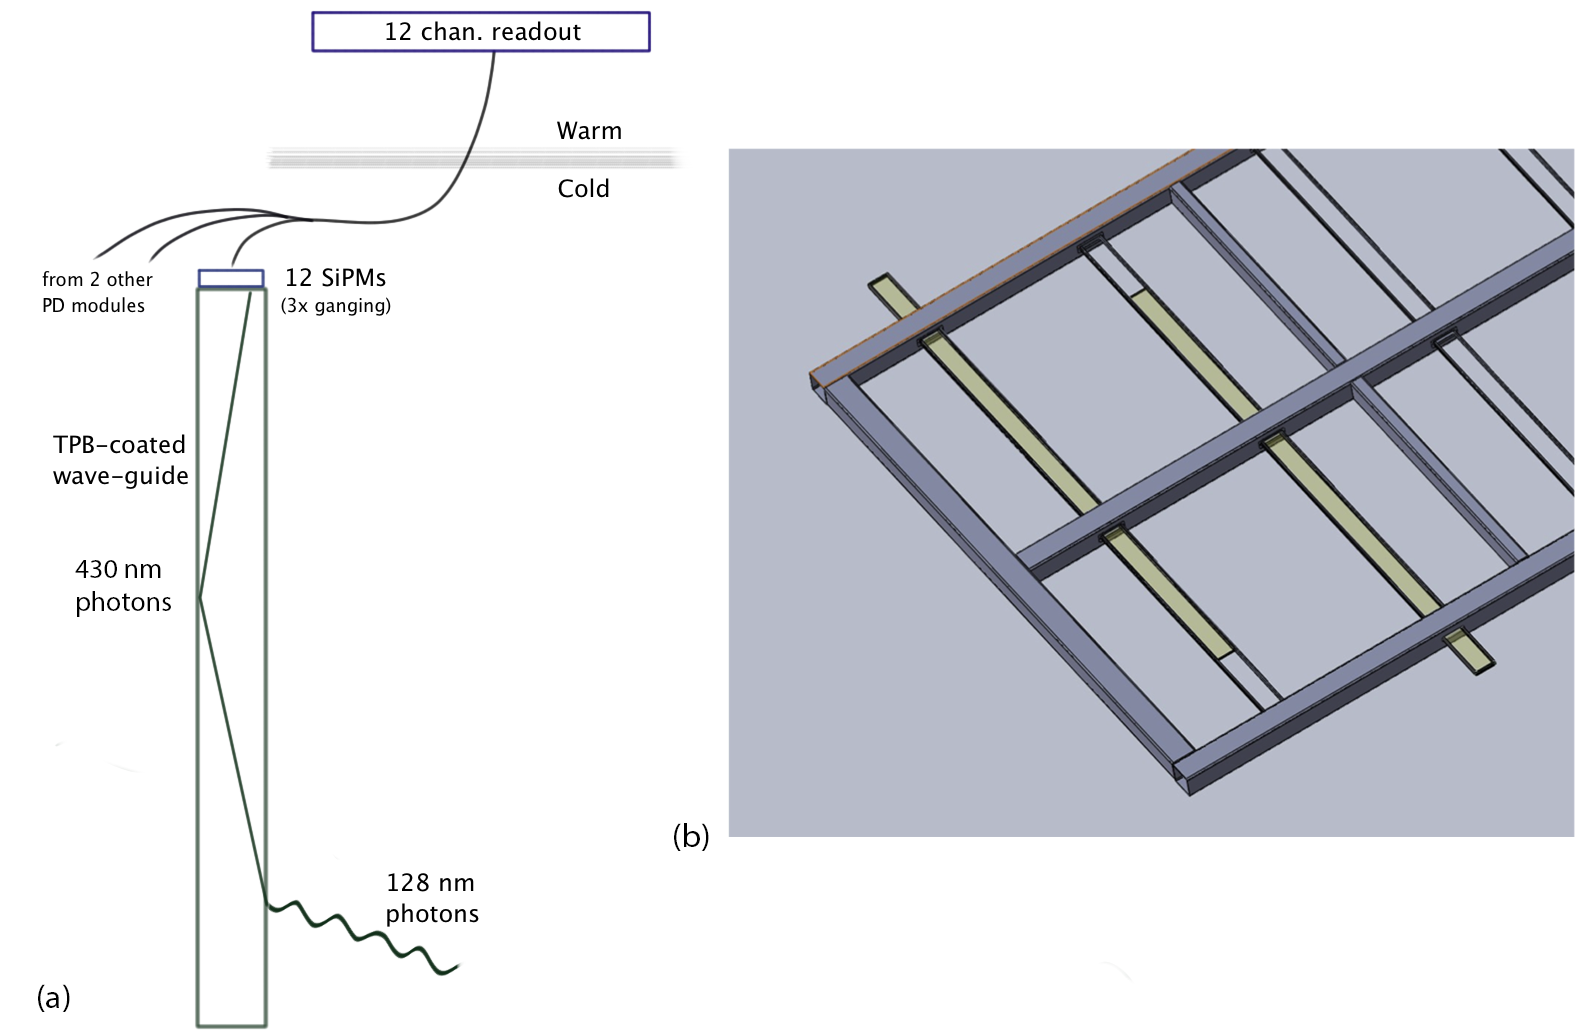
\includegraphics[width=1.0\linewidth]{pd_schem.png}
\end{cdrfigure}

%%%%%%%%%%%%%%%%%%%%%%%%%%
\subsection{Photon detector modules}

Two styles of PDS %photon detector (PD) 
modules are being produced for ProtoDUNE-SP.  
The concepts are very similar, but differ in the number of times the LAr scintillation 
light is shifted.  

The reference design shown schematically in Figure~\ref{fig:PD_RadiatorBar}
has wavelength-shifting radiator plates mounted on a wavelength-shifting light guide.
The plates are coated 
with tetraphenyl-butadiene (TPB) to produce blue ($430nm$) light from the $128nm$ VUV 
scintillation light.  
This blue light is absorbed by a commercially produced wavelength shifting (WLS)
polystyrene bar with Y-11 fluor.  
The bar serves as a light guide to transmit the green light to the photodetector 
mounted at its end.
The radiator plates are captive in mounting blocks that are glued to the WLS bar
at regular intervals as shown in Figure~\ref{fig:PD_radiator_mount}.
\begin{cdrfigure}[Radiator Plate Mounting Blocks]{PD_radiator_mount}
  {Mounting of the radiator plates to the WLS bar for the reference design scheme}
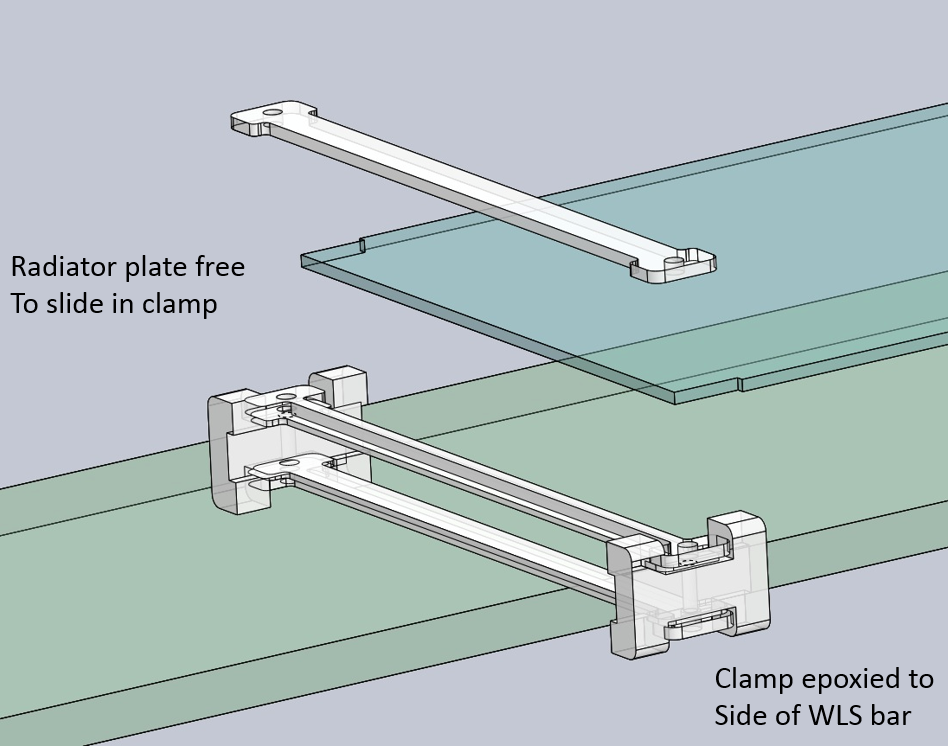
\includegraphics[width=1.0\linewidth]{PD_radiator_mount.PNG}
\end{cdrfigure}

The alternative design uses the same photodetector and mounting, but does not have
any radiator plates mounted on it.  
Instead, the bar is made by dip-coating an acrylic light guide with a solution
of TPB, solvents, and a surfactant to produce a bar with the wavelength shifter coated
on the outside.  
This has advantages in that the expensive fluor is only on the outside where it is
needed, instead of being used as a dopant added during the casting process.  
It also has only one wavelength shifting step, and should be more efficient because
of this.  
Previous work for DUNE with this technique showed that the attenuation length, and
therefore the light yield, would suffer from the coating process, but bars produced with
the latest technique as shown in~\cite{conrad_jinst} have %been shown to have 
avoided
this problem.

%%%%%%%%%%%%%
\subsubsection{Rel Light yield of alternatives}

\fixme{Is this ``Relative'' light yield?}
     % -IU Tallbo -- Denver/Stuart
     %Results of testing
     %Fit to Determine Light Yield
     %Fit/Ratio vs. Distance to determine atten length     
A systematic investigation of promising technologies has been performed on 
many different versions of light collection techniques and guides at the 
TallBo facility at Fermilab.
A test in the summer of 2015 was conducted on the very technologies that 
were chosen for ProtoDUNE-SP. \fixme{Make Ref (DUNE DocDB 138, JINST 11 C05019)}
 

%%%%%%%%%%%%%
\subsubsection{Absolute light yield}
     %Connection to Absolute -- Tallbo-35T  -- Denver Tallbo, Celio,Jonathan,Alex --35T
     %(This could get dropped, or altered depending on status of 35T)
     %Light yield by paddle
     %Comparison to Simulation
     %pe's / MeV 
The testing at TallBo has also been used to connect the relative detector
efficiencies to an absolute light yield that can be used to tune the simulation
yields.  
A Monte Carlo simulation of incident muons in the TallBo dewar, along with ray tracing
of the VUV photons was used to normalize the incident flux of photons impinging on the
light collection paddles.  
The light yield in the measurements were then used to determine the average detection 
probability for a given detector under test.
Light yield data for the two ProtoDUNE-SP paddle types were very similar, justifying
a larger test with additional paddles to detemine the most efficient detector 
technology and allow for further refinements.

%%%%%%%%%%%%%%%%%%%%%%%%%%
\subsection{Radiator/guide lifetime}
     %IU Tallbo and SDSM and T  -- IU design SDSM and T testing  CSU QA/QC
     %Design/Mfr Radiator and guide
     %Design/Mfr dipped guide -- Toups
     %Testing - cryogenic cycling 
     %     rad
     %     guide
     %     dipped guide
     %QA/QC tracking and testing plan  
Several tests have been performed on the light-guide paddles, and testing will 
continue through DUNE to make sure the paddles are sufficiently robust for the
required lifetime.
Light guides based on cast polystyrene and acrylic have been tested 
extensively in LN$_2$ and LAr at Indiana University and in LAr at Fermilab.
No crazing or degradation even after multiple thermal cycles has been seen.
Degradation of the TPB coating has been demonstrated due to UV light.
This was seen in exposure to fluorescent lights and direct sunlight.
Testing with filtered light %that has been filtered 
has been shown to prevent damage
to the TPB coating and will be deployed everywhere the photon detectors
could be exposed.
Additional testing for environmental degradation due to humidity and 
temperature conditions that the components could experience in transit and 
after installation, but before detector filling will continue throughout this
period to determine the required environmental conditions.

\subsection{Experimental Detectors}
While a sufficient number of the two standard arrays are being produced to
fully outfit protoDUNE-SP, it is possible that some will bays will have 
experimental detectors installed in place of the standard arrays.  
One type of detector that is being developed in an attempt to increase the
light detection eficiency is called an ARAPUCA.

The ARAPUCA is a device based on a new technology that should allow to collect photons with a large area window with detection efficiencies at the level of several percent 
while using active photon detectors with much smaller area.
The fundamental idea of the ARAPUCA is to trap photons inside a box with highly reflective internal surfaces, so that the detection efficiency of trapped photons is high even with a 
limited active coverage of its internal surface \cite{arapuca_jinst}.\\

Photon trapping is achieved by using a clever wavelength-shifting technique coupled with the technology of dichroic shortpass optical filters. The latter are multilayer acrylic films that are
highly transparent to photons with a wavelength below a tunable cut-off while being almost perfectly reflective to photons with wavelength above the cut-off. 
A dichroic shortpass filter deposited with two different wavelength shifters (one on each side) will be the core of the device. In particular, it will be the acceptance window of the 
ARAPUCA.\\
The rest of the device will be a flattened box with highly reflective internal surfaces (PTFE, 3M-VIKUITI ESR, \dots), covered by the 
dichroic filter deposited with the two shifters. In principle the box can be filled with any kind of transparent material, since it is inessential to its operation. In our case the material in the 
box is LAr that is known to be perfectly transparent to light.
A fraction of the internal surface of the box is occupied by the active photo-sensors (Silicon Photomultipliers - SiPM) that detect trapped photons.\\

%*****************************FIGURE 1*****************************%
\begin{cdrfigure}[ARAPUCA operating principle]{operating_principle}{Schematic of the operating principle of the ARAPUCA. VUV photons are converted, on the external side of the dichroic filter, to a wavelength L$_1$ below the cut-off. Half of 
them crosses the filter and are converted to a wavelength L$_2$, above the cut-off, by the internal shifter. Since the filter is reflective for wavelengths above the cut-off, the photons are 
trapped inside the box and after few reflections are detected by the SiPM.}
\includegraphics*[width=10.cm]{operating_principle}
\end{cdrfigure}
%***********************************************************************%

The shifters deposited on the two faces of the dichroic filter, S$_1$ and S$_2$ respectively, must have their emission wavelengths, L$_1$ and L$_2$, such that:  
L$_1$ $<$ L$_{cut-off}$$ <$ L$_2$, where L$_{cut-off}$ is the cut-off wavelength of the filter, that is the limit between the region of full transparency (typically $>$ 95\%) and that of full
 reflectivity (typically $>$ 98\%). The side of the filter deposited with S$_2$ is on the internal part of the box.\\
 The operating principle is schematically illustrated in figure \ref{operating_principle}.\\
 
 Two prototypes of the ARAPUCA device have been realized and tested at room and cryogenic temperature (in a LAr evironment) and the effectiveness of the trapping process has been 
 proven in both cases.\\

Two arrays of small ARAPUCAs are planned to be installed inside protoDUNE to test the devices in a real experimental situation and to directly compare their performances with those of the standard guiding bars and other eventual alternative photon detection schemes.\

While the final mechanical design is still under development the arrays will be compatible with the mechanical solutions foreseen for the guiding bars and will have no impact on the construction of the detector. Each of the arrays will replace one bar and will be composed of 8 ARAPUCAs/bar (for a total of 16 devices)  as shown in figure \ref{arapuca_array}.
%*****************************FIGURE 2*****************************%
\begin{cdrfigure}[ARAPUCA array configuration]{arapuca_array}{One ARAPUCA array of 8 devices installed in a APA frame in place of a scintillating bar.}
\includegraphics*[width=8.cm]{APA_ARAPUCA}
\end{cdrfigure}
%***********************************************************************%

Each ARAPUCA will be a teflon box with dimensions of 5$\times$5$\times$1 cm$^3$ with an acceptance window of 5$\times$5 
cm$^2$, will use a filter with cut-off at 400 nm deposited with p-terphenyl and tetraphenyl-butadiene. The trapped light will be detected by 2 SiPM of the same type as the light guide bars.(SensL 60035 - 6$\times$6 mm$^2$ 
active area each).

The readout scheme is expected to gang the SiPMs from two ARAPUCAs (4 sensors) so that each array will require 4 read-out channels. 


%%%%%%%%%%%%%%%%%%%%%%%%%%
\subsection{Sensors}
The planned photodetector is a SiPM.  
The model planned for ProtoDUNE-SP is the SensL C-Series 6~mm$^2$
(MicroFB-60035-SMT) device. These SiPMs have detection efficiency of
41\%; the detection efficiency combines QE and effective area
  coverage accounting for dead space between pixels. While the
C-Series SensL SiPMs are not rated for operation below
$-$40$^{\circ}$~C their performance has been excellent for this
application. 
They have been used in several tests at Fermilab test facilities,
TallBo and Blanche, and were used for the 35-ton prototype detector
as well.  At LAr temperature (89~K) the dark rate is of order 10~Hz
(0.5 p.e. threshold) while after-pulsing has not been an
issue. Extensive testing is underway and will continue, to ensure 
that the SiPMs can reliably survive the stresses associated with 
any thermal cycling in LAr and long-term operation at LAr temperature.

%%%%%%%%%%%%%
\subsubsection{SiPM performance and testing}

All photodetectors for ProtoDUNE-SP will be subjected to testing to determine
\begin{itemize}
\item forward and reverse bias I-V curves,
\item breakdown Voltage,
\item dark current and dark count rate,
\item photodetector gain,
\item crosstalk estimation,
\item response, and
\item bias dependence of parameters.
\end{itemize}
%All SiPMs 
Each SiPM will be tested before mounting on the readout boards to determine
if the part meets the specifications in a warm test.  After mounting to
the readout board all items will be tested both warm and cold (cyrogenic 
temperature) to determine the operating characteristics as when %they will be 
installed at the ProtoDUNE-SP detector, and during QA/QC tests on the PDS modules.

In addition to these tests, the photodetectors will be tested for their
response to light signals from an LED with appropriate wavelength.
These tests will be sensitive enough to determine if one of the three SiPM
elements in parallel is not functioning.


%%%%%%%%%%%%%
\subsubsection{SiPM Lifetime}
Studies have been performed to investigate the ageing of the SiPM devices over time at 
cryogenic temperatures as a result of exposure to light.
Currently, a set of 63 devices have been tested for degradation.
The SensL Series C SiPMs showed no evidence for degradation in their 
performance in the equivalent of 250 years of exposure underground at DUNE. 
The tests investigated SiPM response, noise rate, cross-talk probability, and
gain.
Detailed test results can be seen on DUNE-doc-904. (Make a reference) 
Additional long-term testing with an expanded throughput are beginning
now.

A passive aging test was initiated in March 2015 to follow the
behavior of six SensL series C SiPMs in a simulation of the benign
DUNE environment. These SiPMs have been continuously in the
dark in LN$_2$ for over 425 days. Four properties have been monitored:
dark noise rate, cross talk probability, breakdown voltage, and gain
slope. So far, the measurements show that there
have been no significant changes in these properties during the
duration of the test.
Detailed test results can be found in DUNE-doc-905. (make a reference)

%In addition to these tests, the C series SiPMs have been used for the
%readout of modules that were built to test the relative light yield of
%different light guide technologies in the TallBo tests.  In this testing 
%An additional 80 SiPMs have been used successfully in this testing that 
%required their deployment at cryogenic temperatures in a vessel with 
%similar conditions to what they will be exposed to in the experiment.
%None of the SiPMs deployed in this way have failed.


In addition to these tests, an additional 80 of the C series SiPMs have been used for the
readout of modules that were built to test the relative light yield of
different light guide technologies in the TallBo tests.  %In this testing 
This testing 
required the SiPMs' deployment at cryogenic temperatures in a vessel with 
similar conditions to those expect to be present during experiment operations. 
This testing has been successful; none of the SiPMs deployed in this way have failed.

%%%%%%%%%%%%%%%%%%%%%%%%%%
\subsection{Mechanical design and installation}
  % -- CSU  -- Dave
  %  Mechanical Design Mounting 

The PDS system is configured as a set of \textit{modules} that are mounted on the APA frames.  A PDS module is
the combination of one light guide (also called a ``bar'' due to its
shape) and 12 SiPMs, as shown in Figure~\ref{fig:PD_overview}~(a).  %To enable this, the the reference design for mounting the PDs onto the
The reference design for the APA frames calls for ten PDS modules per APA, approximately 2.2-m long,
86-mm wide and 6-mm thick, equally spaced along the full length of the
APA frame, as shown in Figure~\ref{fig:PD_overview}~(b). 
The light guides are inserted into the APA frame on rails gliding on their radiator
plate mounting blocks, as shown in Figure~\ref{fig:PD_mounting_inslide.PNG}.

\begin{cdrfigure}[Diagram of PDS installation into APA frame]
  {PD_mounting_inslide}{Rendering of the installation of a PDS module
    into an APA frame, shown just before it comes to rest on the inside face
    of the APA tube.}
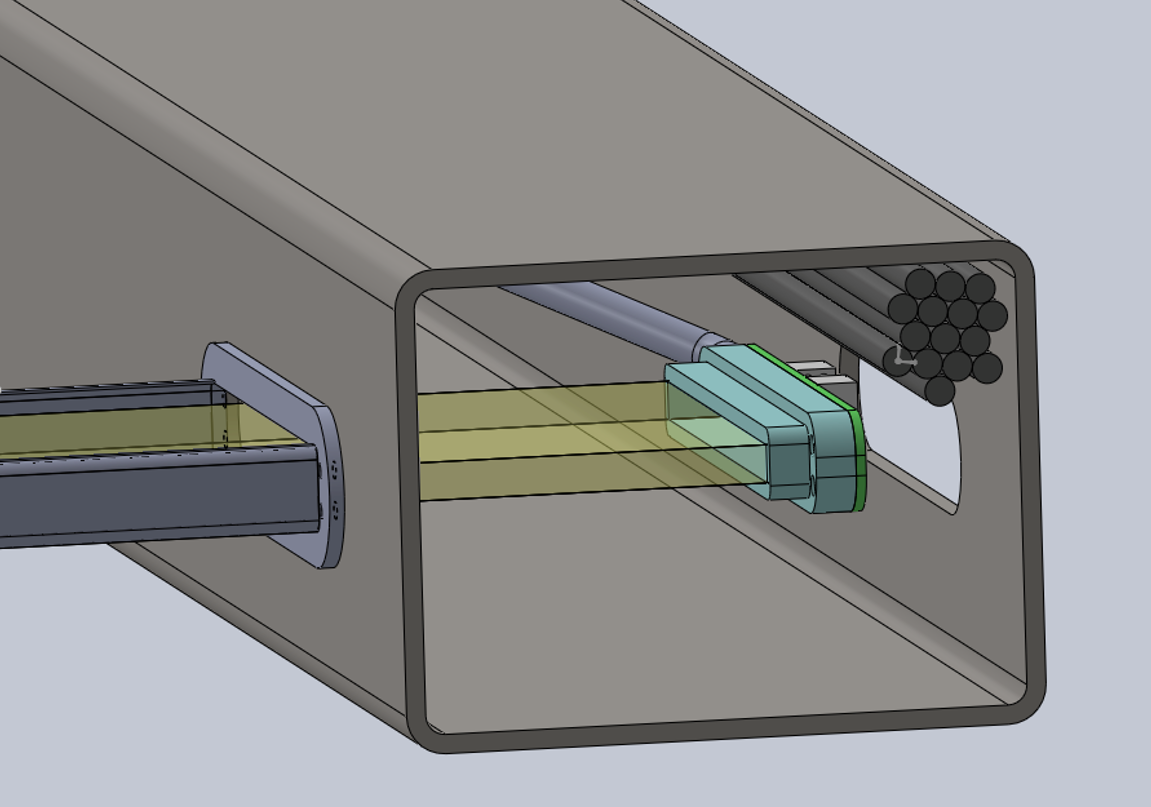
\includegraphics[width=0.50\linewidth]{PD_mounting_inslide.PNG}
\end{cdrfigure}

The system has been prototyped and test fitted with a module at CSU 
as shown in Figure~\ref{fig:PD_flat_installtest}.
\begin{cdrfigure}[Photo of PD mock installation]
  {PD_flat_installtest}{Photograph of the installation
    test of a mock PDS module in a 1/5 section of an APA frame.}
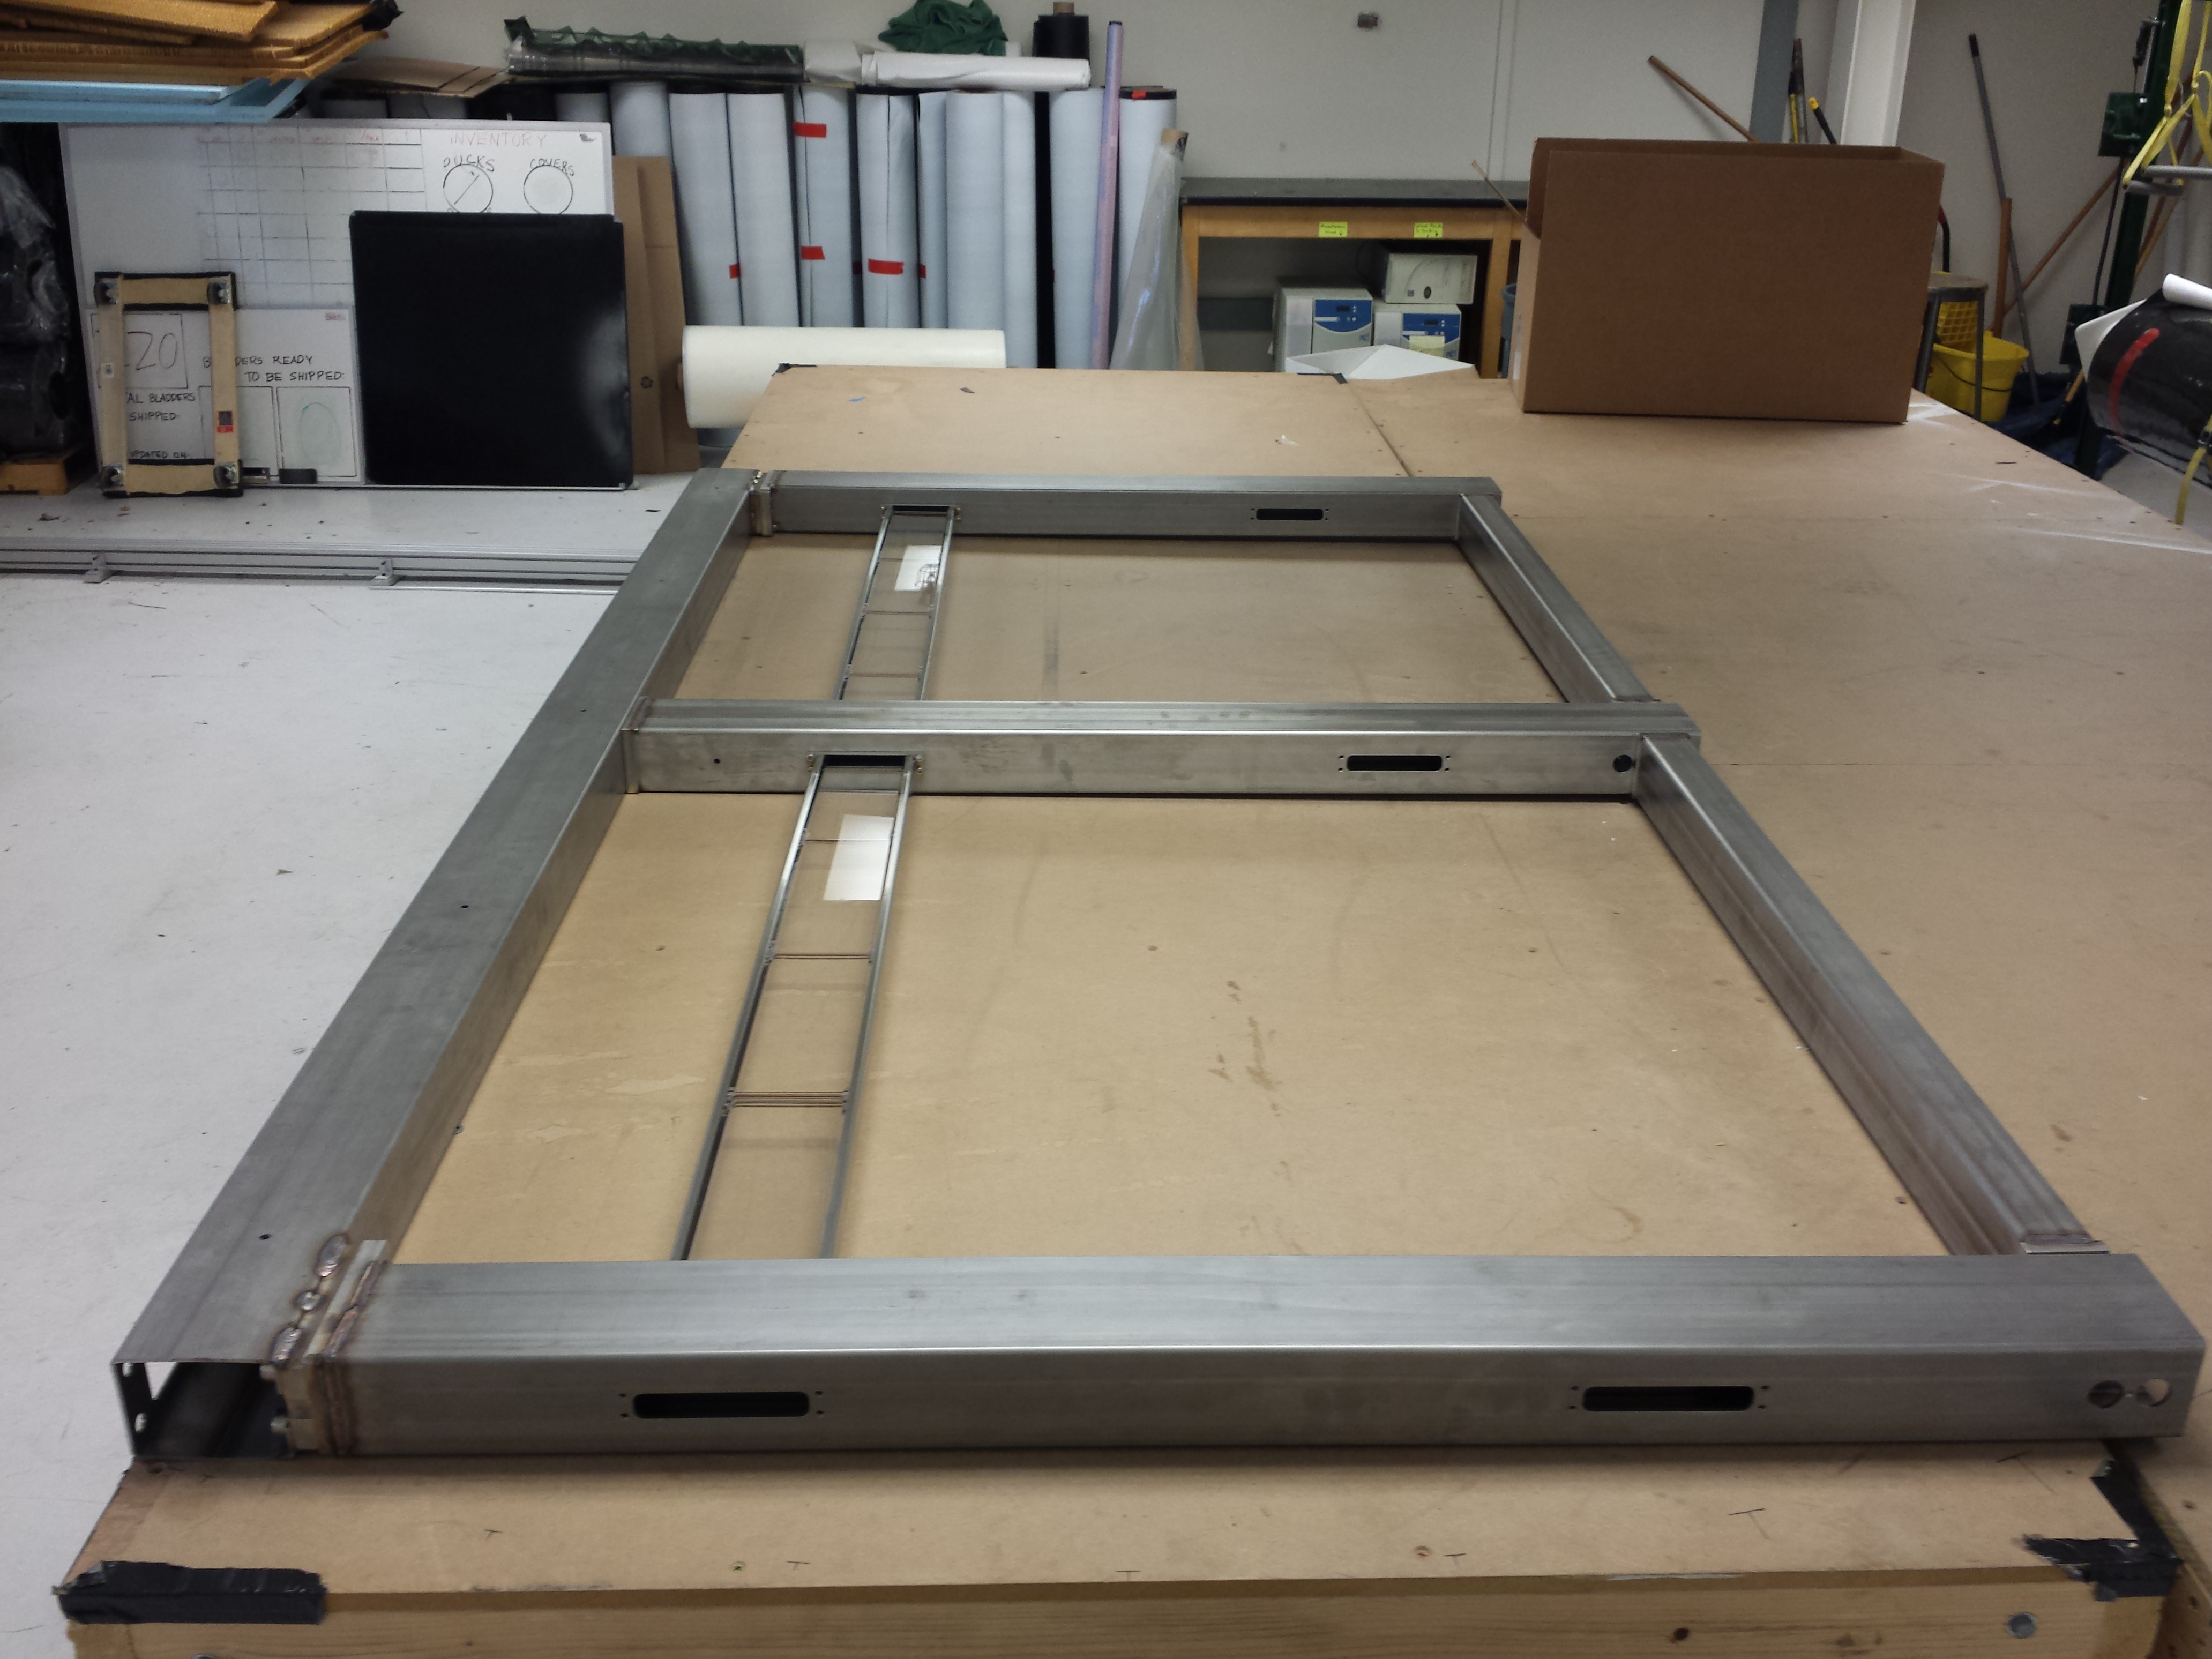
\includegraphics[width=0.50\linewidth]{pd_flat_installtest.jpg}
\end{cdrfigure}

  %   Mechanical Design SiPM mounting board

Each photon detector has a single SiPM mounting board with 12 surface-mount SiPMs 
mounted on the face as in Figure~\ref{fig:PD_SiPM_PCB_front}.
Four groups of $3$ SiPM elements will go to a single 
channel of readout electronics in order to reduce the cost of the readout.
The board is held close to the bar, without touching, by four screws that go into 
tapped holes on the end mounting block that is glued to the bar.  
The mounting block assembly is shown in Figure~\ref{fig:PD_endblock_mnt}.
The circuit board also has holes at each end for mounting to the APA frame.  
\begin{cdrfigure}[SiPM mounting board with 12 SiPMs mounted]
  {PD_SiPM_PCB_front.PNG}{Photograph of a SiPM mounting board
    with the full complement of 12 SiPMs installed on the board.}
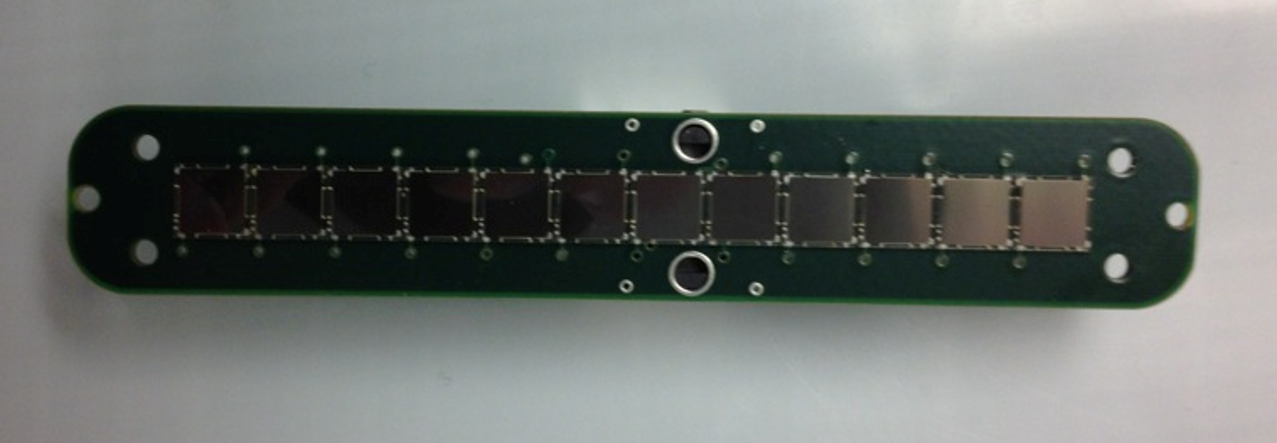
\includegraphics[width=0.50\linewidth]{PD_SiPMMountPCB_front.PNG}
\end{cdrfigure}
\begin{cdrfigure}[SiPM mounting board attached to PDS module]
  {PD_endblock_mnt.PNG}{Rendering of the the SiPM mounting board
    installed on the end of the PDS module before insertion.}
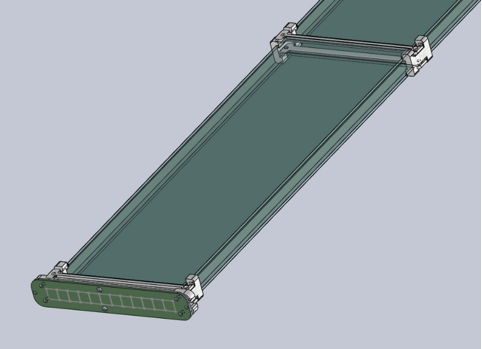
\includegraphics[width=0.50\linewidth]{PD_endblock_mnt.PNG}
\end{cdrfigure}

  %   Mechanical Design Cabling

The cabling plan for the system has one cable with four shielded twisted pairs 
connected to each SiPM mounting board via the surface mount RJ-45 connector
shown mounted on the back of the readout PCB in 
Figure~\ref{fig:PD_SiPMMountPCB_back.PNG}.  
\begin{cdrfigure}[Readout board with RJ-45 connector]
  {PD_SiPMMountPCB_back}{Photograph of the SiPM readout PCB with the 
    RJ-45 connector for the cable.}
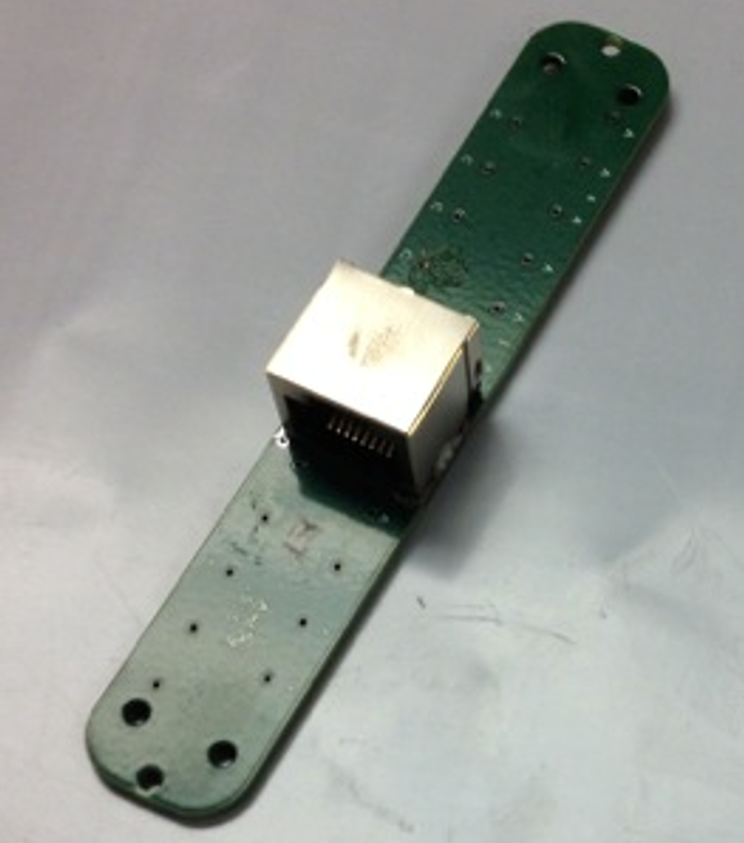
\includegraphics[width=0.50\linewidth]{PD_SiPMMountPCB_back.PNG}
\end{cdrfigure}
The cables run through the APA tubing to the top of the APA frame as seen
in Figure~\ref{fig:PD_cable_intube}.
The cable bundles are installed and connected to each PD 
after the PD has been installed into the slot.
\begin{cdrfigure}[Cables in APA frame]
  {PD_cable_intube}{Diagram showing the routing of the PDS cables
    through the APA frame.}
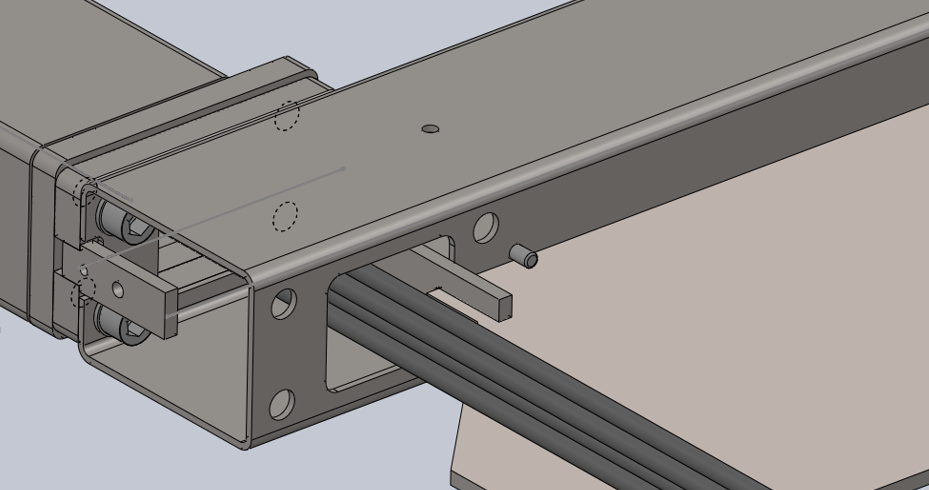
\includegraphics[width=0.50\linewidth]{PD_cable_intube.PNG}
\end{cdrfigure}

%%%%%%%%%%%%%%%%%%%%%%%%%
%\subsection{PD Calibration}

\subsection{Photon Detector UV-Light Monitoring System}
\label{sec_pd_calib}

%Items relevant to the PDS calibration are the fast and slow components of the light, photon propagation including scattering and reflections, impact of N$_2$, E-field strength, 
%and the energy range of interest. A calibration system that addresses these issues has to be both comprehensive and cost-effective, and has to be tied to the overall 
%calibration system for ProtoDUNE-SP, which includes both charge and scintillation light calibration techniques. 
%In addition, there is a need to evaluate relative efficiencies of multiple PD units and monitor response and stability of the system as a function of time.

A UV-light-based monitoring system that will serve to monitor the relative performance and time resolution of the system has been designed. % and is described here.
The system will consist of a set of UV LEDs as light sources in the VUV wavelength range, coupled to quartz fibers, to transmit light from outside the detector volume to desired locations at the CPA within the TPC.
Light diffusers located at the CPA surface will uniformly illuminate the APA area with photon-detector system (PDS) elements.
The light sources located and fired externally, with fibers running into the cryostat to diffusers that will emit light from the CPA to the APA. 
For the ProtoDUNE-SP cryostat at the surface at CERN, the UV light system will be complementary to cosmic ray muon 
tracks and Michel electrons as means of calibration. In terms of light sources the measurements will be performed with an UV (245-280) light source.
The UV light essentially mimics physics, although at a different wavelength starting from the wavelength-shifter conversion, 
light guide propagation, photo-sensor detection and the front-end electronics readout.
	
The external UV-light monitoring system is designed with the following goals:
				
\begin{itemize}
\item Simple to implement (no active components within PD/APA, such as LEDs or fibers mounted within APA).
\item Uniformly illuminates APA surface with the light diffused from CPA locations.
\item Has a potential to be adapted for deployment in a large Far Detector in the future
\end{itemize}

In terms of technical requirements the system needs to:
\begin{itemize}
\item provide light levels down to a single p.e. at individual photon-detector channels,
\item provide higher light levels to test linearity of the PDS,
\item provide variable pulse width to test the time resolution of the photon detector response, and
\item uniformly illuminate the APA area of the detector for relative monitoring of the PDS channels
\end{itemize}

%Leon stopped fixing here 8/31

Figure~\ref{fig:fig-c-1} illustrates the system design schematically. The system consists of a 1U rack mount Light Calibration Module (LCM) sitting outside the cryostat. The LCM generates light pulses that propagate through a quartz fiber-optic cable to diffusers at the CPA to distribute the light uniformly across the photon detectors mounted within the APA.  ProtoDUNE-SP will have five light 
diffusers on the CPA plane: one in the center and four diffusers close to the CPA corners, as illustrated in Figure~\ref{fig:fig-c-2}. 
%
 \begin{cdrfigure}[UV-light monitoring system]{fig:fig-c-1}{Concept of the UV-light monitoring system for the photon detector in liquid argon.}
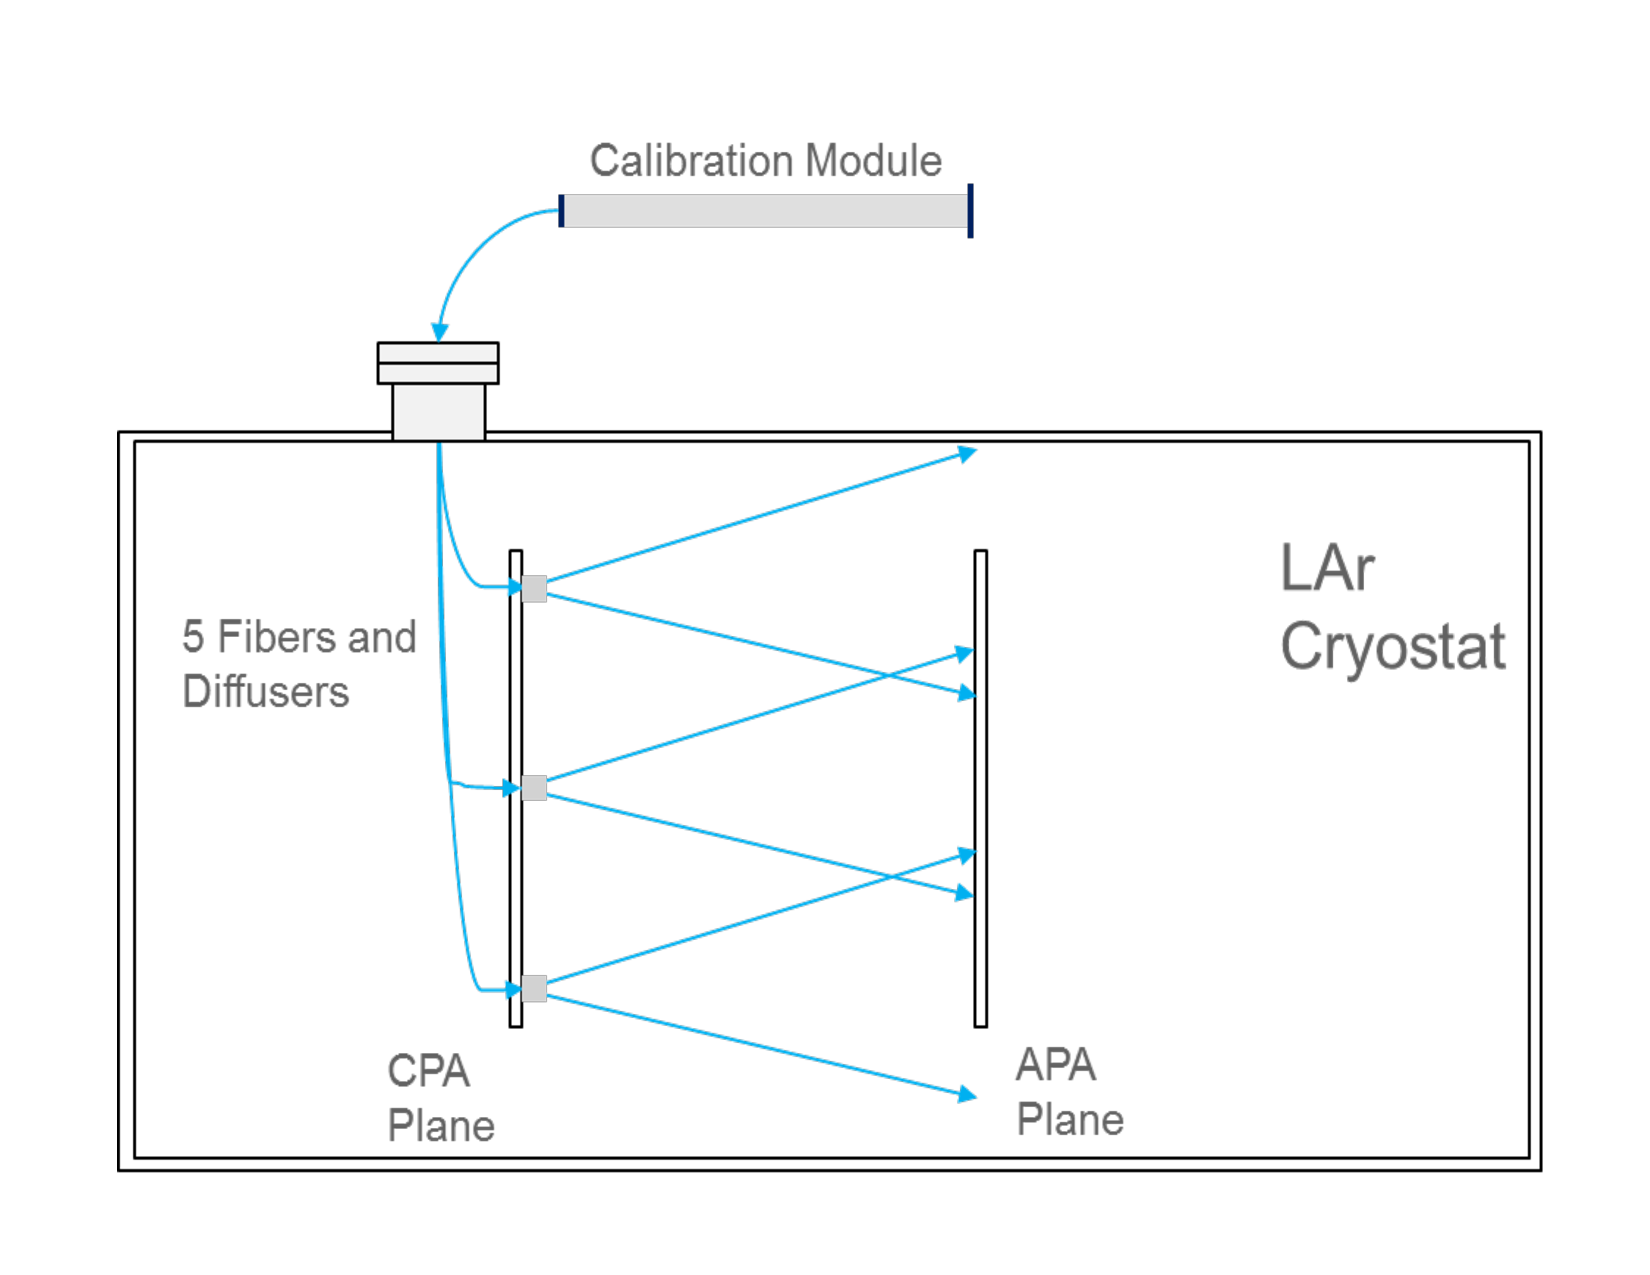
\includegraphics[angle=0,width=10cm,height=7cm]{calPD_concept-from-35ton.pdf}
\end{cdrfigure}
%
%
\begin{cdrfigure}[Deployment of PDS UV-light monitoring system]{fig-c-2}{The diffuse light is emitted from diffusers (top and bottom left figure) mounted at five CPA locations, indicated by arrows (right figure). 
The UV light from the light Calibration Module to diffusers is transported through quartz fiber.}
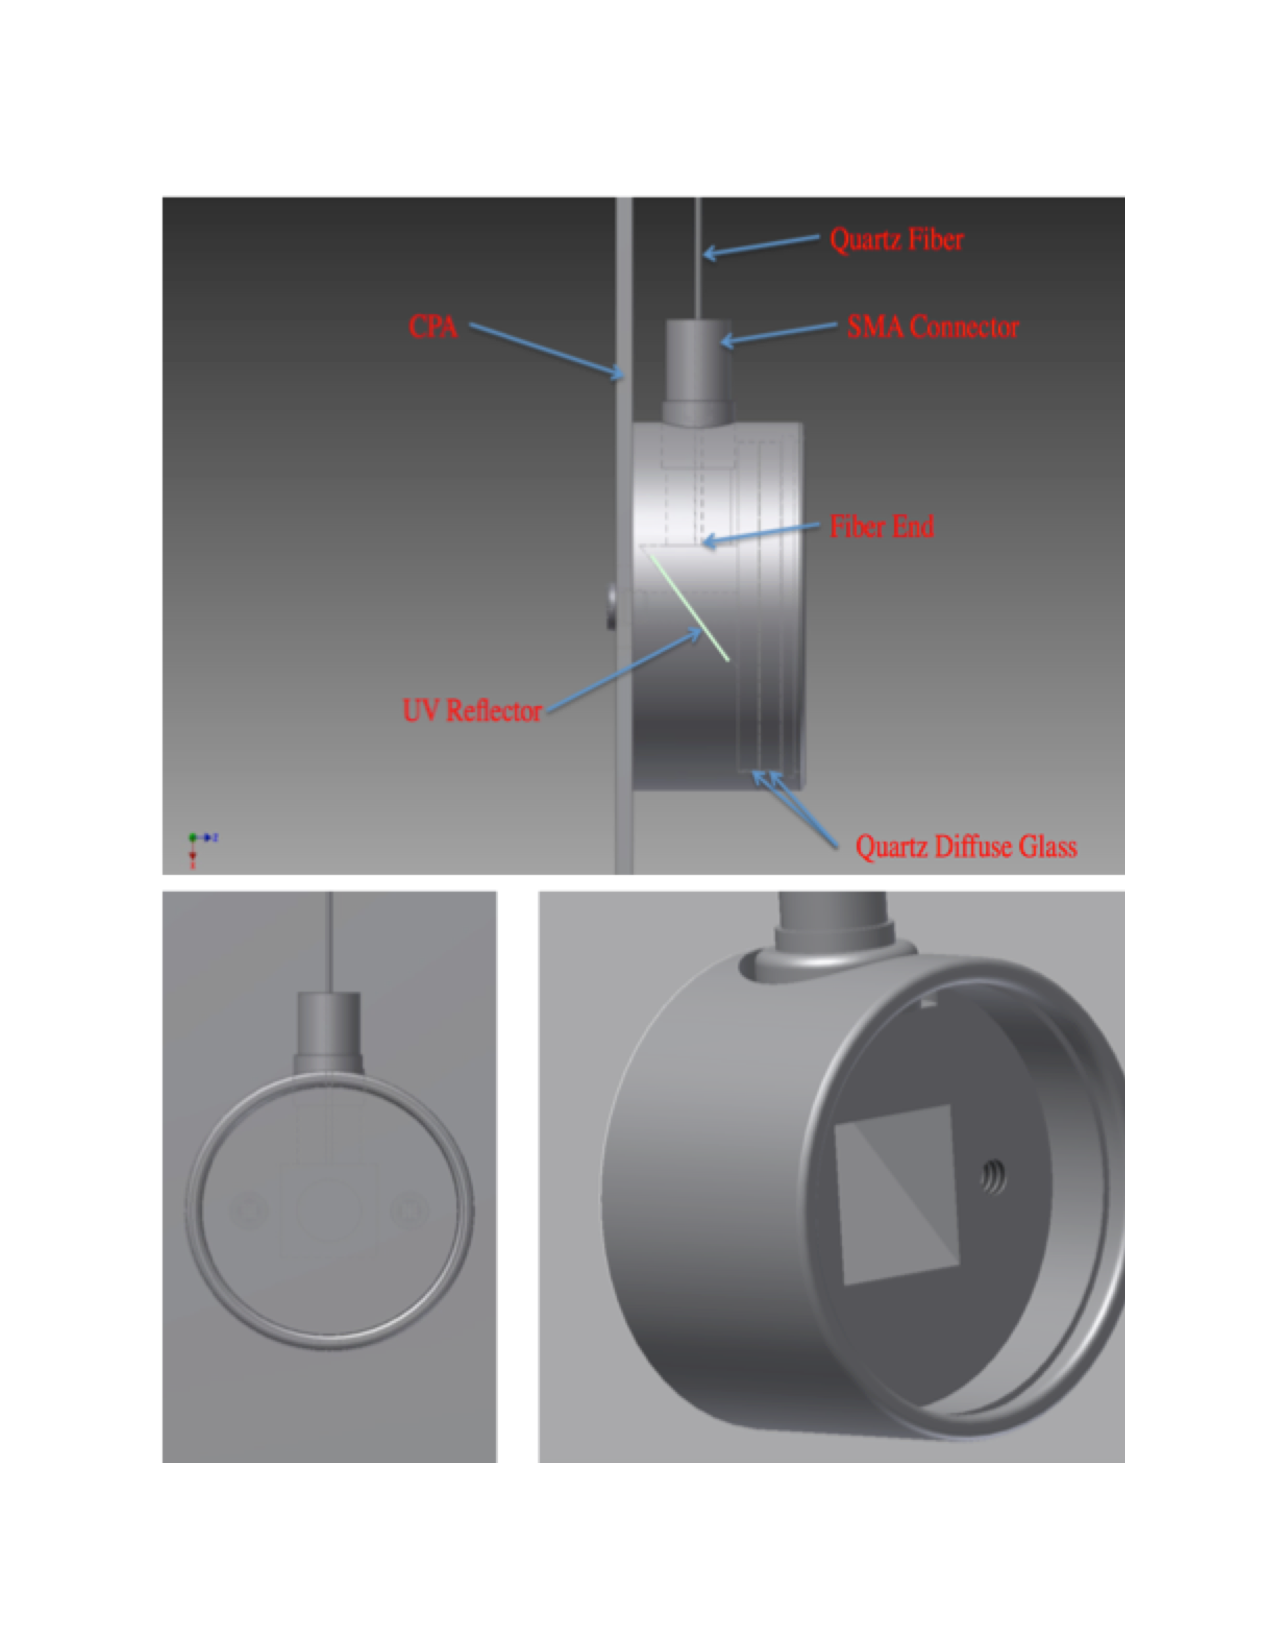
\includegraphics[angle=0,width=0.4\textwidth]{calPD_Calibration_diffuser_system_protoDUNE_slide_left_half.pdf}
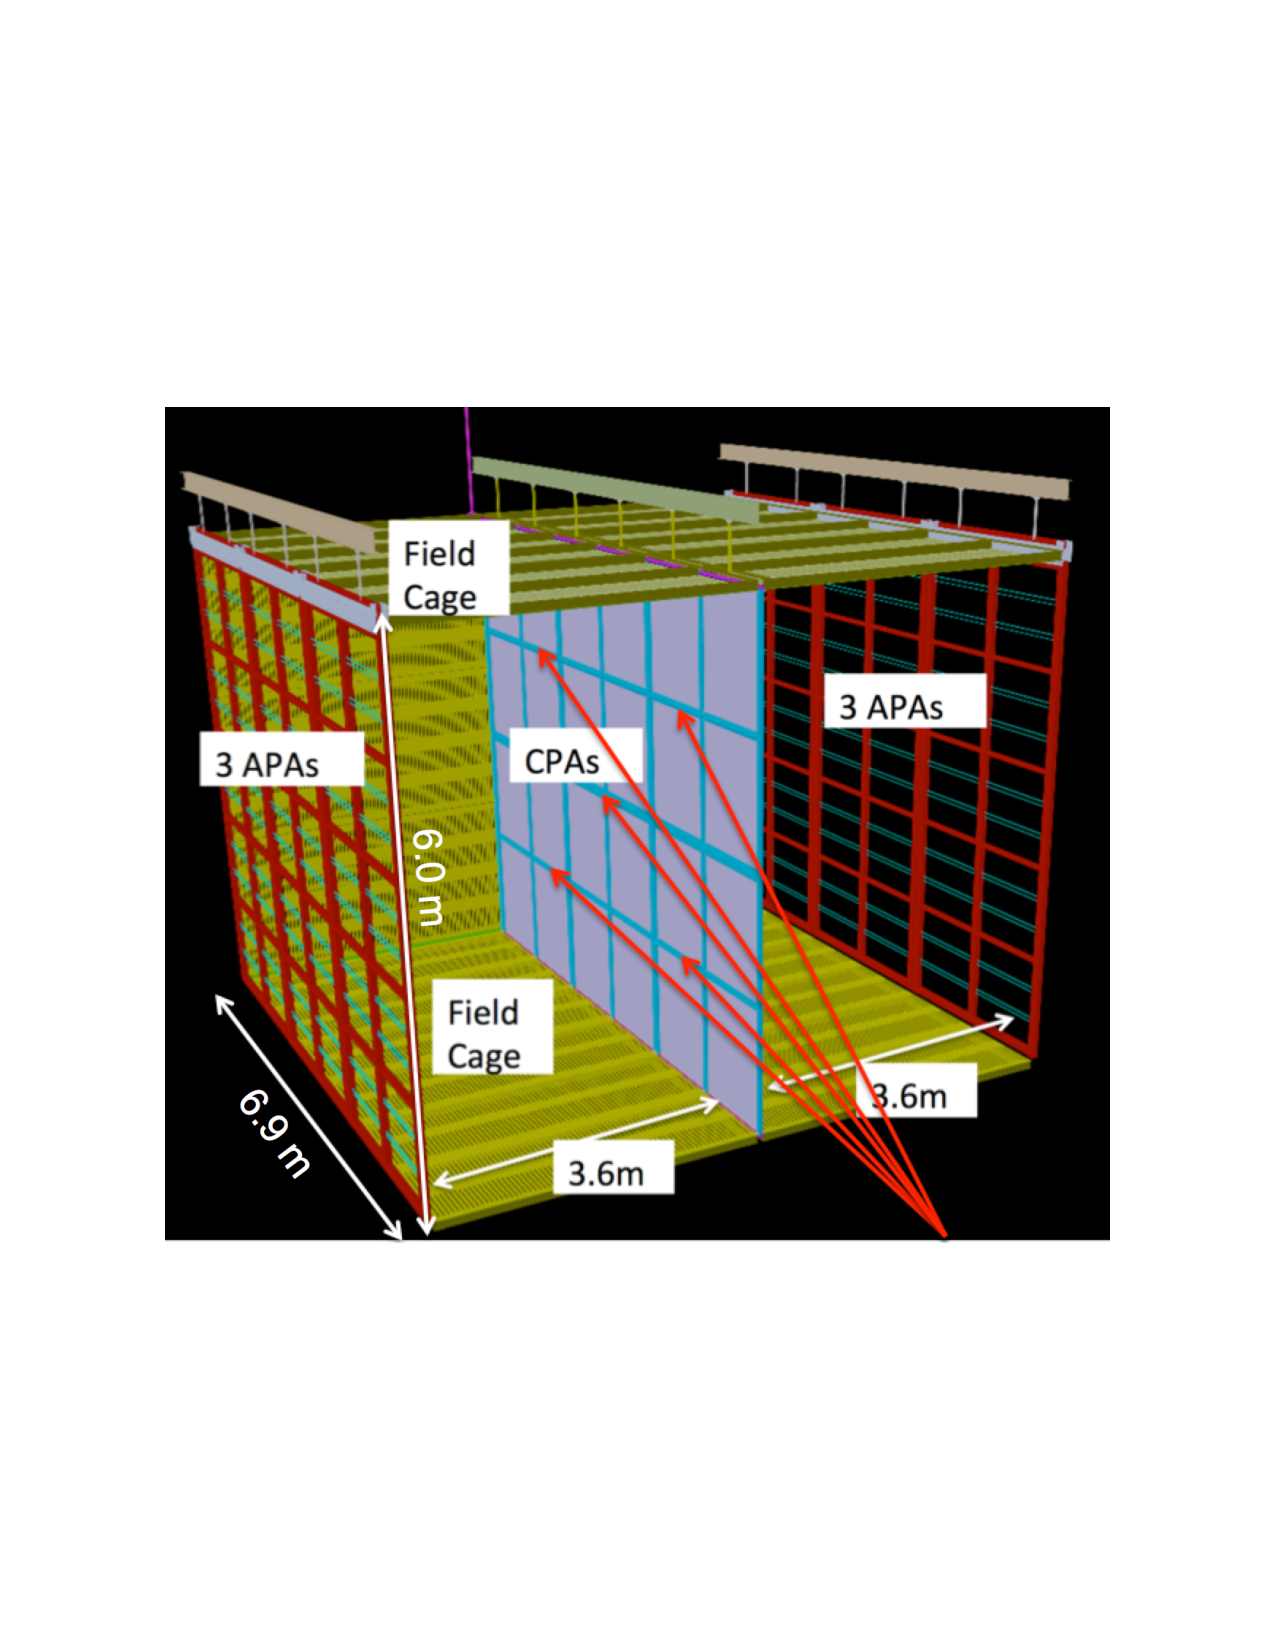
\includegraphics[angle=0,width=0.55\textwidth]{calPD_Calib_diffuser_locations_protoDUNE.pdf}
\end{cdrfigure}

\fixme{left hand figure's text is way too small}
%
%
For the 280-nm light a simulation of the designed diffuse light monitoring system has been performed using TracePro, a generalized 3D light ray-tracing program with the ability 
to include bulk optical properties such as absorption, fluorescence, and birefringence in addition to surface properties such as scattering and reflection. 
As an example, Figure~\ref{fig:fig-c-4} shows simulated light distributions at an APA surface for the cases of the VUV light emitted by either the central diffuser only (left figure), 
or by the outer four diffusers simultaneously (right figure). 

%
\begin{cdrfigure}[UV-light monitoring illumination calculation]{fig:fig-c-4}{Simulated light distributions of at the APA location for the cases of the VUV light emitted by either the central diffuser only (left figure), or by outer four diffusers simultaneously (right figure).
The simulation estimate has been obtained for 35-ton detector and scaled by to 3.6 m CPA - APA distance at ProtoDUNE-SP.}
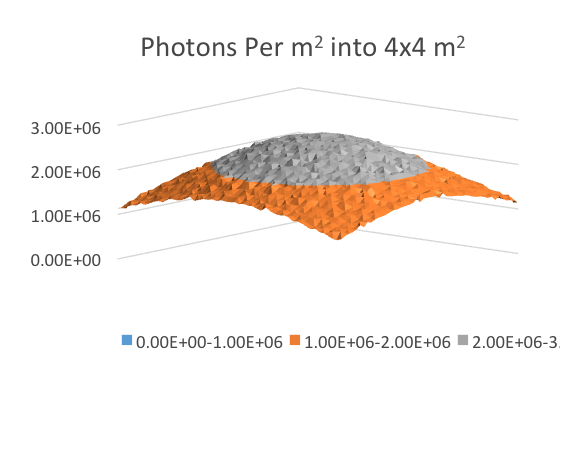
\includegraphics[angle=0,width=6.5cm,height=6cm]{calPD_4mx4m-area-3point6m-away-quantified.png}
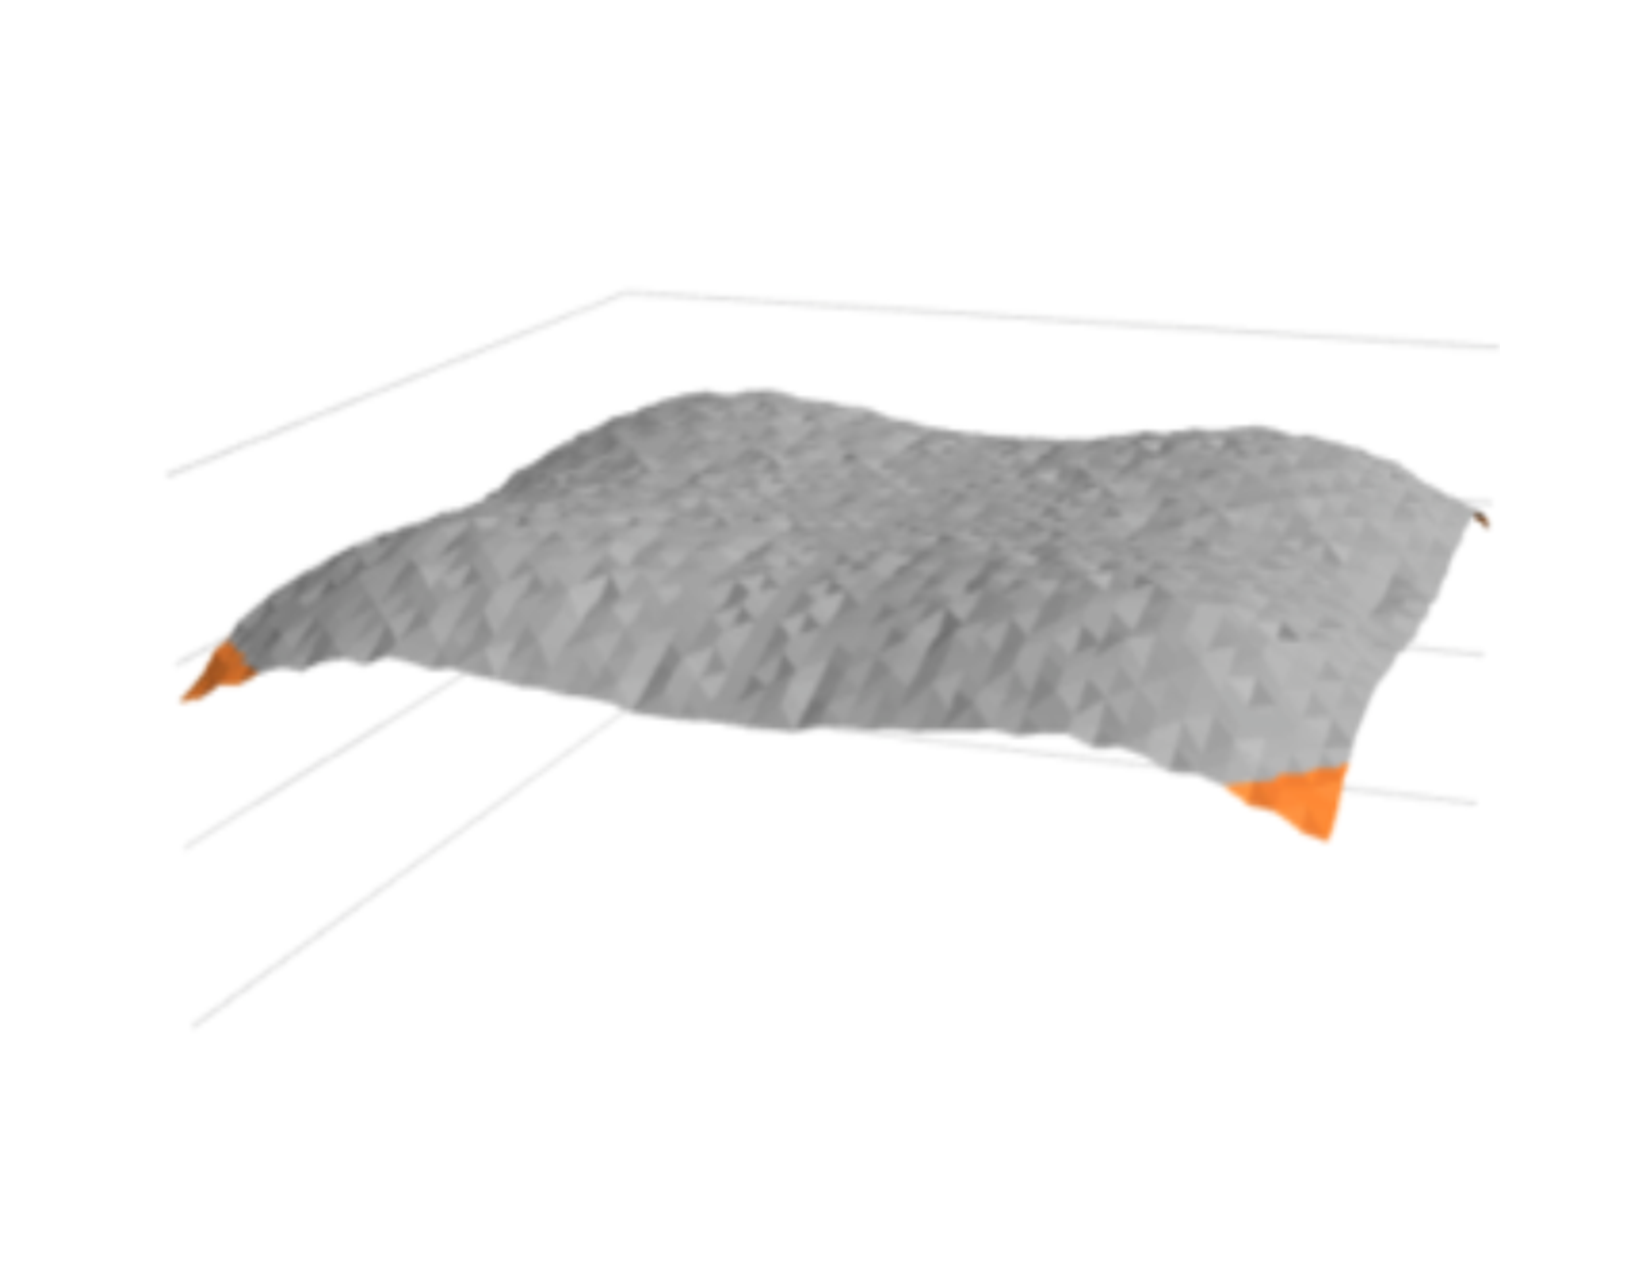
\includegraphics[angle=0,width=6.5cm,height=6cm]{calPD_figR.pdf}
\end{cdrfigure}
%

The LCM as well as the full prototype of the light monitoring system system has been built, tested and successfully operated with 35-ton LArTPC at Fermilab. The LCM shown in Figure~\ref{fig:fig-c-3}
utilizes the logic and timing control of the photon-detector readout electronics ("SSP") unit.  
An SSP board was repackaged into a deeper rack mount chassis that accommodates a new internal 
LED Pulser Module (LPM) and an additional bulk power supply. The LPM utilizes five digital outputs from the SSP board to control the LPM pulse and its duration.  
These outputs are derived from the charge injection control logic within the SSP's FPGA.  
The even-channel SiPM bias Digital to Analog Converters (DACs)
are used to control the LPM pulse amplitude.  
The adjacent odd channels are used to read out a reference photodiode used for pulse-by-pulse monitoring of the LED light output.  
The output of the monitoring diode may be used to normalize 
the response of the SiPMs in the detector to the monitoring pulse.

%
 \begin{cdrfigure}[]{fig:fig-c-3}{Photon detector light calibration module (LCM) front (left) and back (right) ends.}
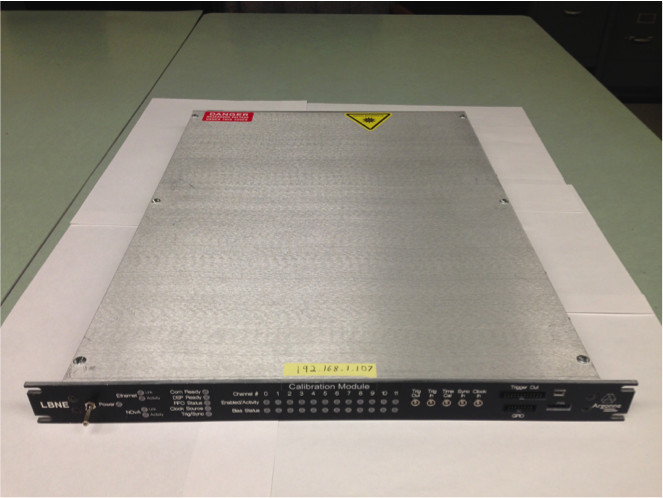
\includegraphics[angle=0,width=7cm,height=4.5cm]{calPD_LCM_front.png}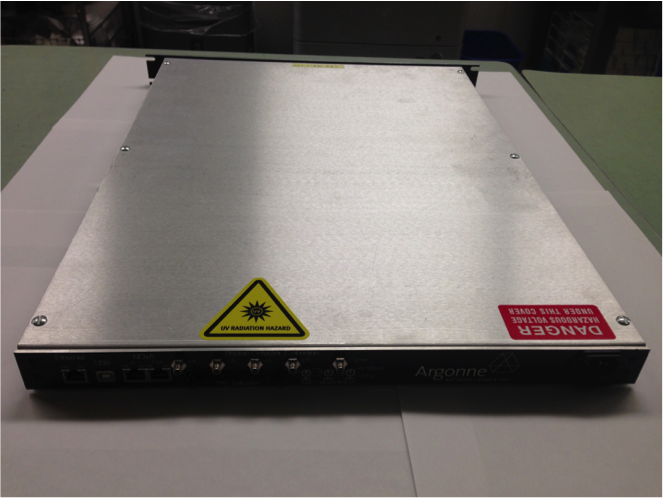
\includegraphics[angle=0,width=7cm,height=4.5cm]{calPD_LCM_back.png}
\end{cdrfigure}


The data from the 35-ton test is currently being analyzed. %As en example of the system tests in former 35-ton detector in 
Figure~\ref{fig:fig-wf} shows SSP waveforms collected as a response to the light  monitoring system % described here.
%This data has been collected 
in liquid argon, with the TPC powered-on, and at the nominal value of drift high-voltage.  
%at 35-ton detector. 
The length of optical fiber cables used %with the 35-ton detector 
was $\sim$22 m total, including external fibers (7 m), and fiber feed-through and internal fibers (15 m).

%
 \begin{cdrfigure}[Detected UV-light monitoring system light pulses]{fig:fig-wf}{Photon detector light pulses detected by readout electronics. Recorded waveforms have range from few photo-electrons (left figure), to tens of photo-electrons (middle figure), to hundreds of photo-electrons (right figure).}
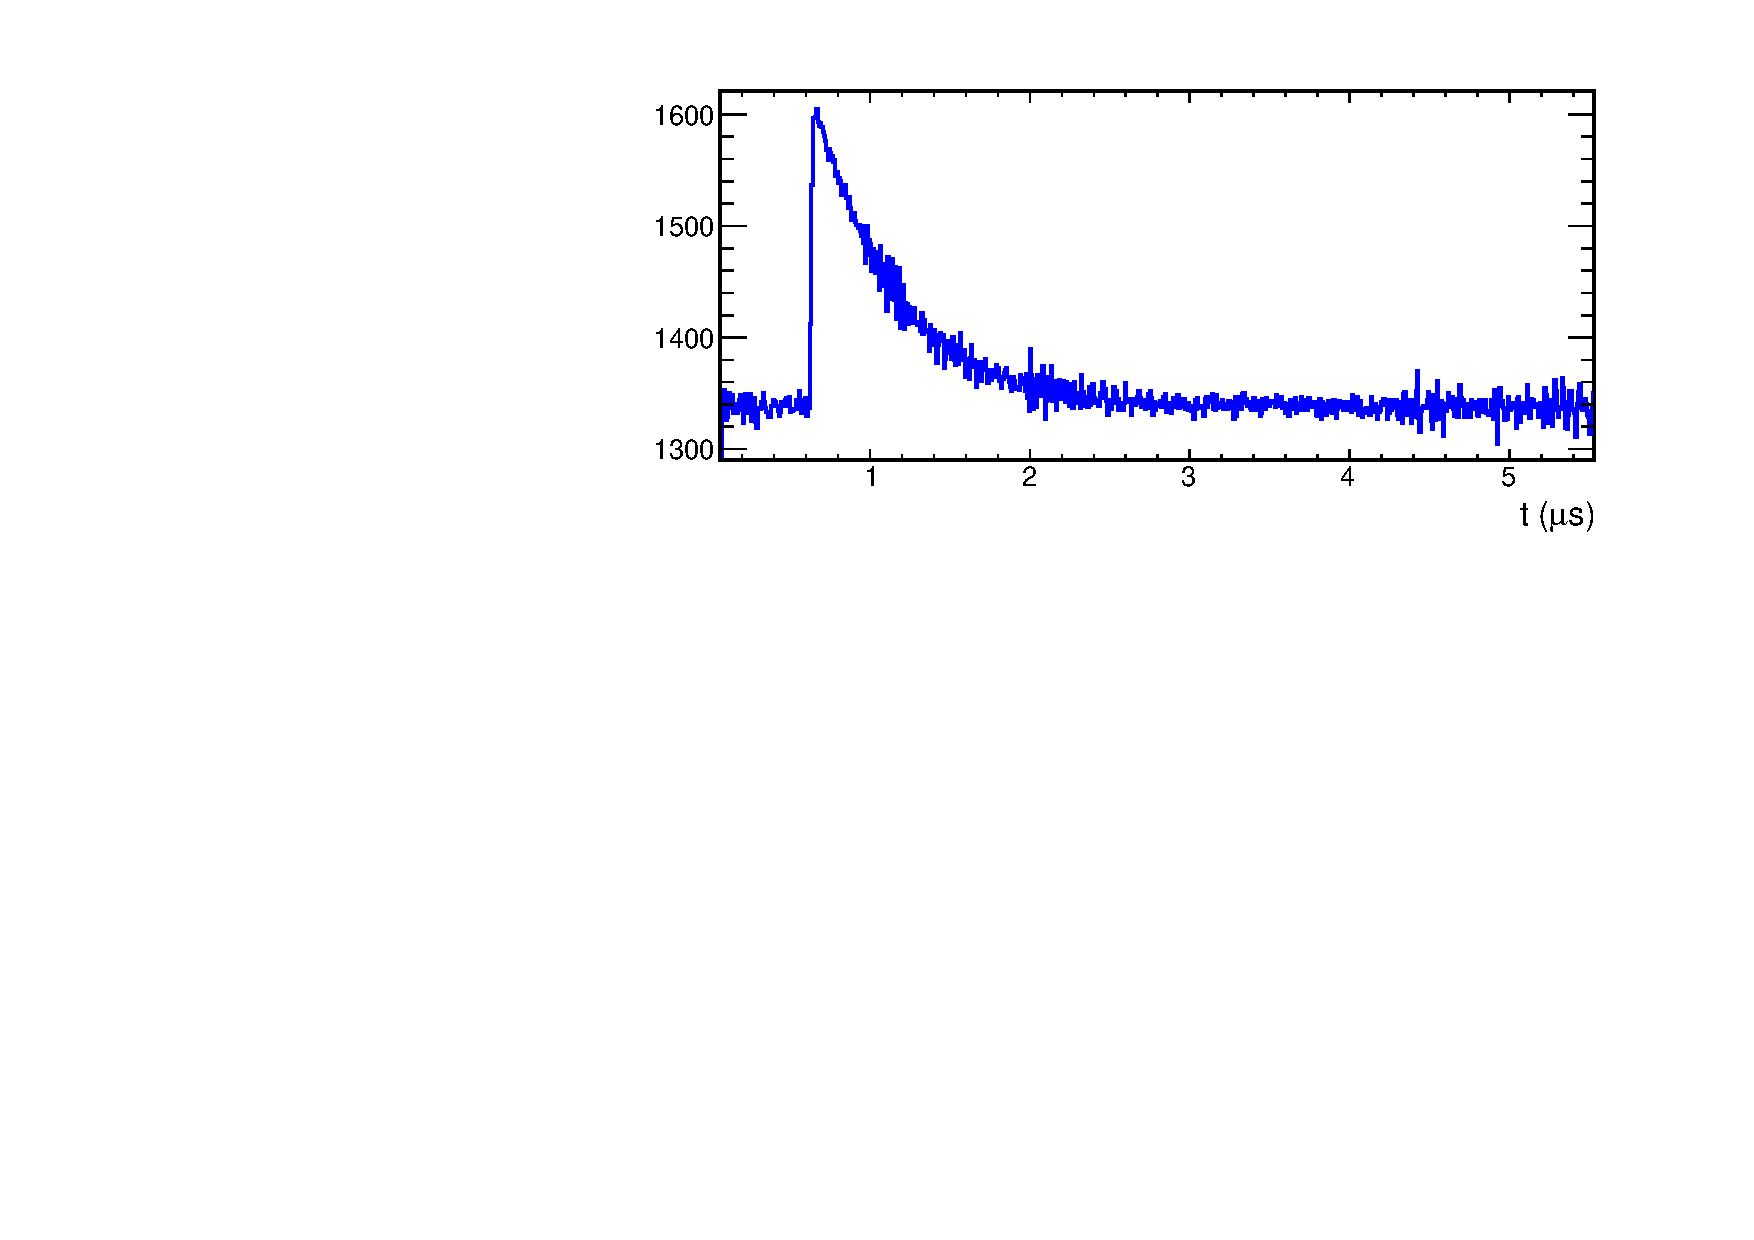
\includegraphics[angle=0,width=5cm,height=4cm]{calPD_example_ch21_run18573.pdf}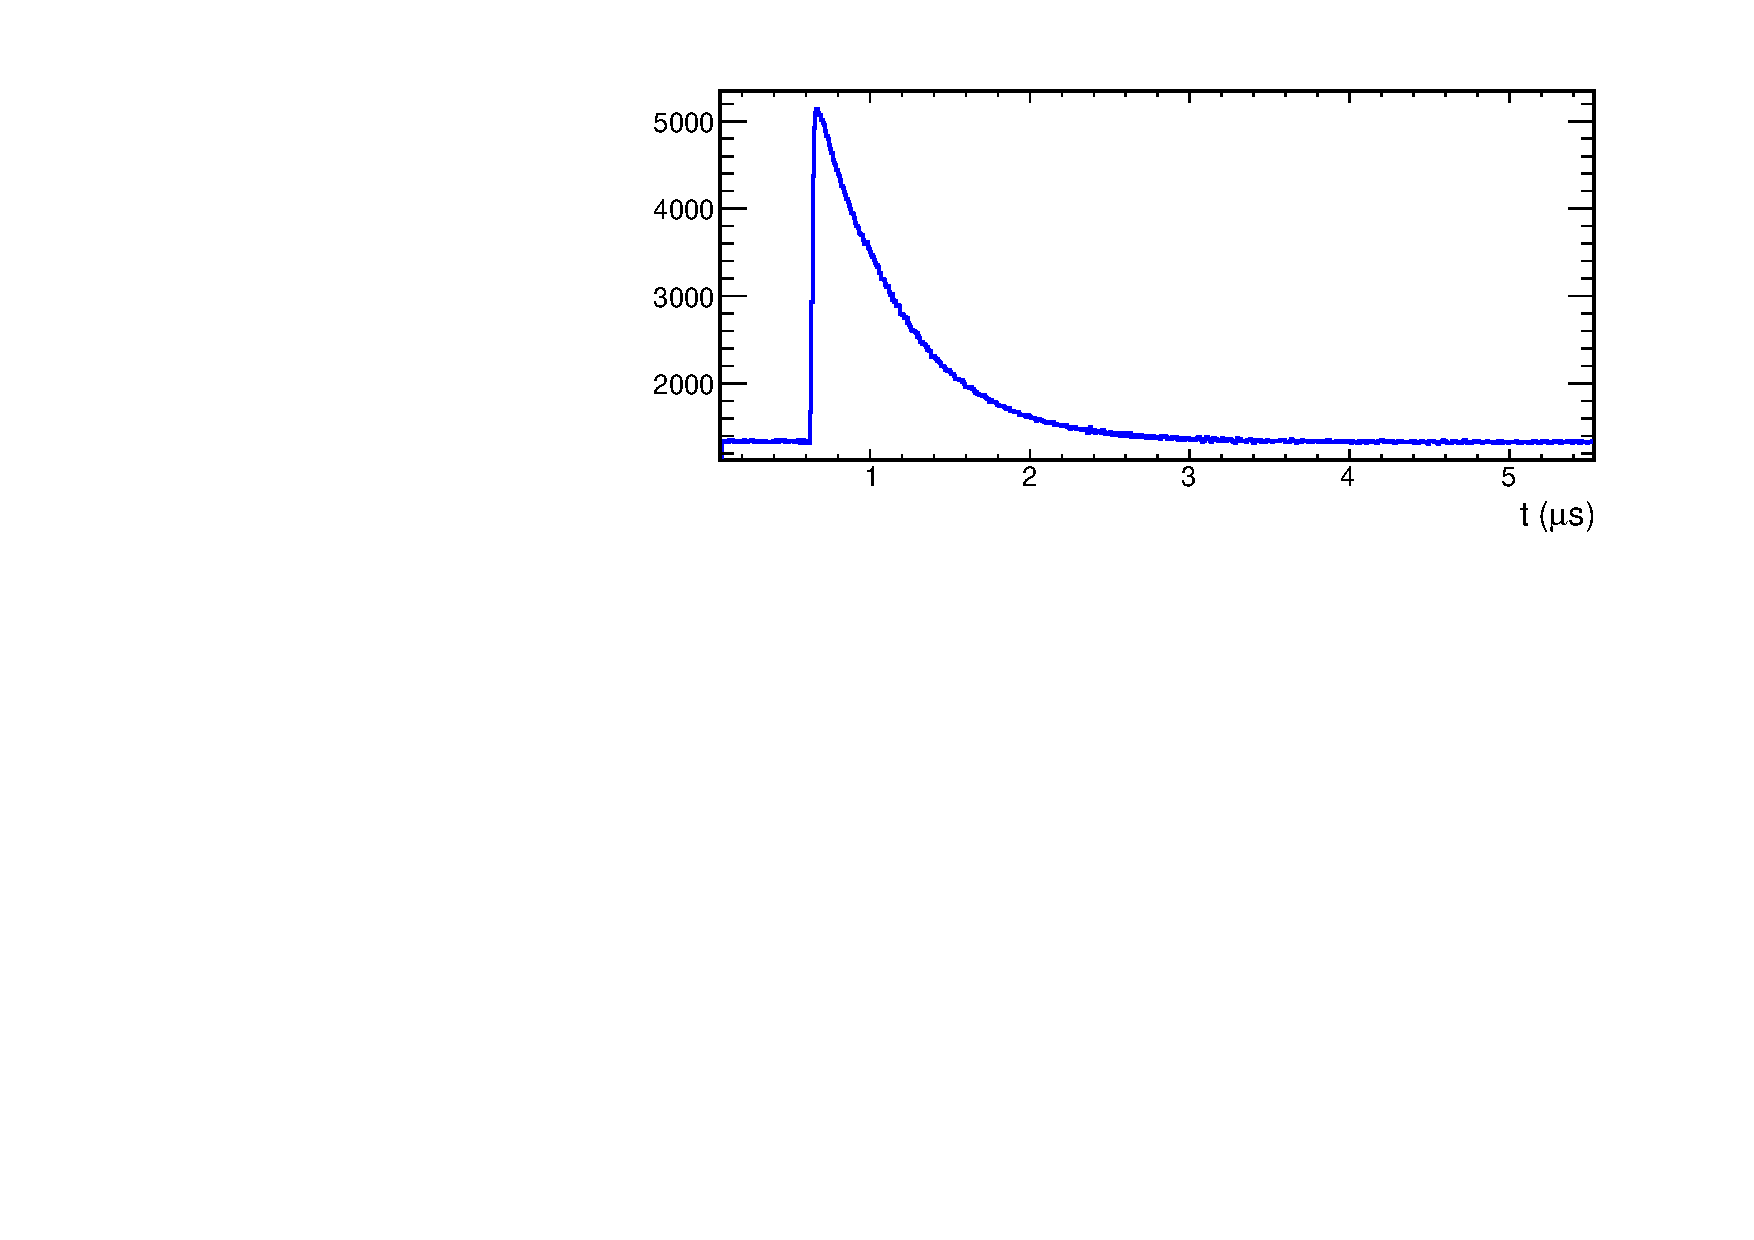
\includegraphics[angle=0,width=5cm,height=4cm]{calPD_example_ch21_run18574.pdf}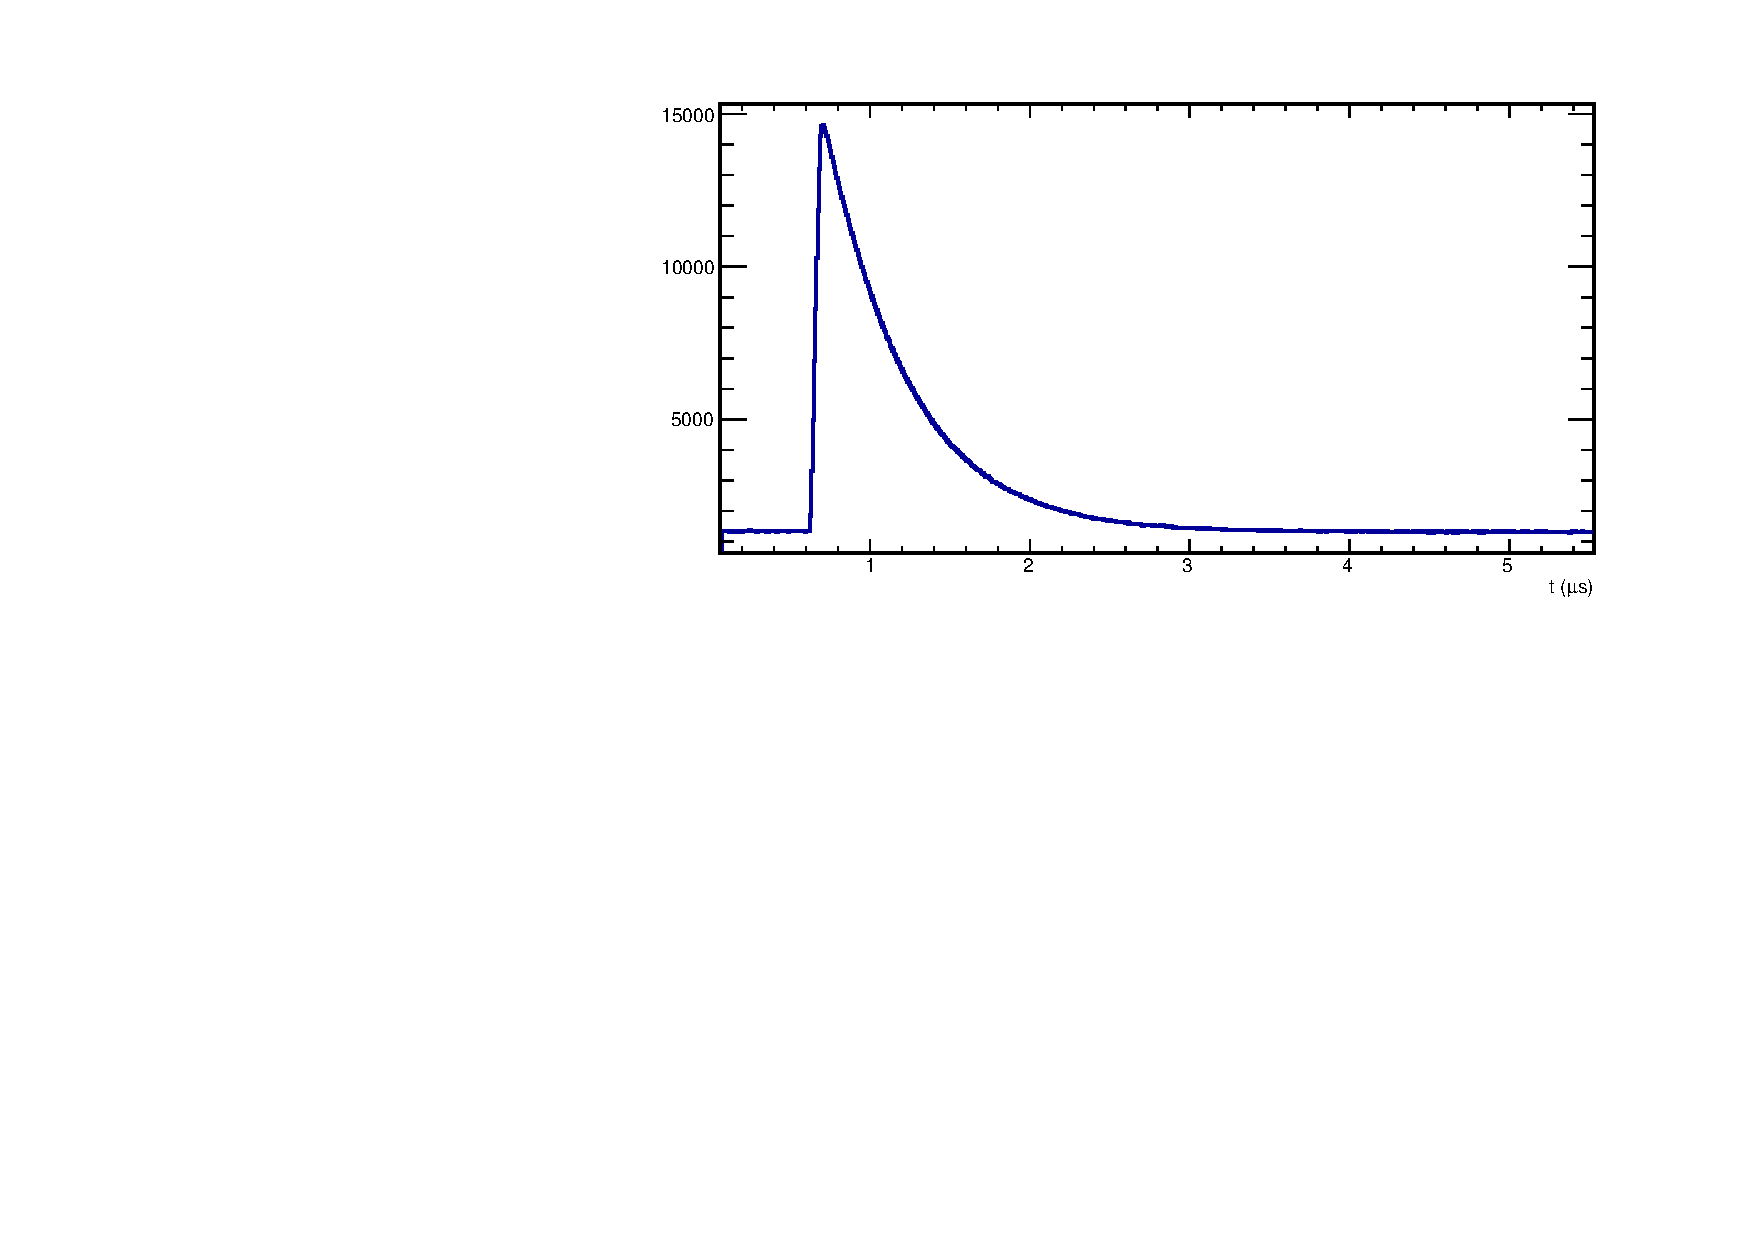
\includegraphics[angle=0,width=5cm,height=4cm]{calPD_example_ch21_run18572.pdf}
\end{cdrfigure}
%
In the DUNE prototypes (e.g., the ProtoDUNE-SP) and in future DUNE far detector modules it will be important to 
verify the proper function of photon-detector components
at various stages of the detector operation. 
Periodic light-source deployments will monitor the system's stability as a function of time. A change in relative difference of UV light responses would point towards potential wavelength shifter instability, 
or changes in SiPM gain and/or collection efficiencies. %Much of the same monitoring is expected to be doable with cosmic rays in the ProtoDUNE-SP (at surface), with 
Periodic LED monitoring runs will be complemented 
with cosmic-ray data tracked by an external hodoscope. 
%With the ProtoDUNE-SP detector one could use a well-defined muon trajectory defined by the hodoscope geometry and monitor the number of PEs per MeV of deposited charge. 
A well-defined muon trajectory defined by the hodoscope geometry could be used to monitor the number of p.e.'s per MeV of deposited charge, which in turn 
%The number of p.e.'s per photon-detector channel from the well defined muon track 
could be used as a calibration constant. This technique will likely be unusable 
%However, 
for the deep underground DUNE detectors since the cosmic ray flux may be inadequate. % for timely monitoring of the photon detectors.
	Two sets of calibration runs are planned for the ProtoDUNE-SP detector: 
\begin{enumerate}
\item Monitoring runs with four outer diffusers run simultaneously, in order to
   \begin{itemize}
   \item measure response of PDS channels in multi-p.e. range and get integrated number of event samples for each channel (for maximum light output);
   \item test  the dynamic range from 1 p.e. to maximum number of p.e.'s; and
   \item repeat runs periodically to trace any changes in channel response.
    \end{itemize}
\item Runs with central diffuser only, in order to
   \begin{itemize}
   \item perform initial test runs that will reveal malfunctioning channels, if any;
   \item perform timing measurements with the 10--50-ns pulses; and
    \item verify time resolution of the PDS.
   \end{itemize}
\end{enumerate}

The controlled source of light %described here 
in this monitoring system will be used to perform time offset and time resolution measurements.  
Many effects contribute to a finite time resolution, relative time offset of photon-detector channels, scintillation time constants, 
photon conversion with wavelength shifter, photon propagation through photon-detector paddle, SiPM jitter, and FEE resolution. 
Most of these effects are constant and can be individually 
measured on the bench.  The UV light monitoring system will monitor overall stability of the photon detector in both time
and amplitude.


%%%%%%%%%%%%%%%%%%%%%%%%%
\subsection{QC Procedures}
QC procedures and tracking are being developed in a separate document.
  %   QA/QC tracking for components
% This could be a whole document of its own.


